\subsection{More examples}

We will now instantiate our algorithm for a couple more examples, illustrated in \figureref{examples}.

\begin{figure}
  \centering
  \subfigure[Hidden Markov Model] {
    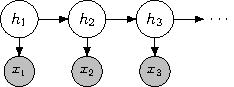
\includegraphics[width=0.45\columnwidth]{figures/hmm.pdf}
    \label{fig:examples-hmm}
  }
%  \subfigure[Directed grid model] {
%    \label{fig:examples-grid}
%    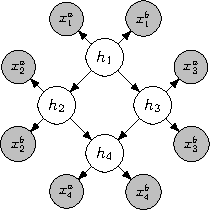
\includegraphics{figures/grid.pdf}
%  }
  \subfigure[Tree model] {
    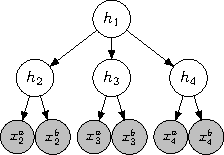
\includegraphics[width=0.45\columnwidth]{figures/tree.pdf}
    \label{fig:examples-tree}
  }
  \caption{Additional examples of models learnable using \LearnMarginals}
  \label{fig:examples}
\end{figure}

\paragraph{Hidden Markov Model}

In this example (\figureref{examples-hmm}), we assume that
  $\Pr(x_i|h_i) = O  ~\forall i$  and that $\Pr(h_{i+1} | h_i)
  = T ~\forall i$ (i.e. we have parameter sharing).
Note that while the first (and last) hidden variables $h_1, h_T$ in the
  sequence are not bottlenecks, they still have exclusive views ($x_1$ and
  $x_T$ respectively) whose parameters we know because they share
  parameters, $O$.
In step 1 of our algorithm, we use the bottleneck $h_2$ with views $x_1,
  x_2, x_3$ and solve $O$.
In step 2 of our algorithm, we can recover $\pi$ by solving for the
  unary clique $\{h_1\}$ and recover $T$ from the clique $\{h_{1},
  h_{2}\}$.

\paragraph{Latent Tree Structure}

In the latent tree structure (\figureref{examples-tree}), let the
  parameters be $\Pr(h_i) = \pi$, $\Pr(h_i | h_1) = T ~i \in \{2,3,4\}$
  and $\Pr(x^a_i | h_i) = \Pr(x^b_i | h_i) = O ~i \in \{2,3,4\}$.
Note that while $h_1$ is not directly connected to an observed variable,
  it is still a bottleneck, with views $x^a_2, x^a_3, x^a_4$.

In step 1, we recover the parameters $O$ from the bottleneck $h_2$ with
  views $\{x^a_2, x^b_2, x^a_3\}$. We also recover the conditional moments
  $\mOpp{2}{1}$, $\mOpp{3}{1}$, $\mOpp{4}{1}$ for $h_1$. 
In step 2, we can recover $\pi$ from the clique $\{h_1\}$, using any
  one of views (they are all exclusive). 
To recover $T$ from the clique $\{h_1, h_2\}$, we use the views $x^a_2$
  (exclusive to $h_2$) and $x^a_3$ (exclusive to $h_3$). Note that while
  $x^a_3$ is also a view for $h_2$, $x^a_3$ is independent of $h_2$ given
  $h_1$.

\paragraph{Aggregating observations}
We describe two practical considerations to use samples more efficiently.
Firstly, if we have multiple exclusive views for a hidden variable,
  intuitively, it is better to aggregate over them. 
For example, consider a hidden variable $h_1$ with multiple exclusive
  views $x_1$ and $x_2$.
With the method of moments perspective, to learn the marginal
  distribution over $h_1$, one must solve the following reconstruction
  problem, 
\begin{align*}
  \hat Z_{h_1} &= \arg\min_{Z_{h_1}} \half \|Z_{h_1}(\mOpp{1}{1}) - M_1 \|^2 + \half \|Z_{h_1}(\mOpp{2}{1}) - M_2 \|^2,
\end{align*}
which does not have a closed form solution. 
In contrast, this naturally fits into the convex optimization framework, where $\hat Z_{h_1}$ will now be,
\begin{align*}
  \hat Z_{h_1} &= \arg\min_{Z_{h_1}} \sum_{\vx \in \sD} \log Z_{h_1}( \mOpp{1}{1}[x_1] \odot \mOpp{1}{1}[x_1] ),
\end{align*}
where $\cdot$ denotes element-wise multiplication.
An important note to make is that \TensorFactorize only returns
  a solution up to permutation; if $\mOpp{1}{1}$ and
  $\mOpp{1}{2}$ do not belong to the same bottleneck (e.g. $x^a_2$ and
  $x^b_2$ in \figureref{examples-tree}), then some
  care must be taken to ensure they have the same labelling.

Secondly, we can exploit parameter sharing by aggregating over
  disjoint sets of observed variables. 
For example, in \figureref{examples-hmm}, we can aggregate the statistics for
  bottlenecks $h_i$ with views $\{x_{i-1}, x_{i}, x_{i+1}\}$ before
  running \TensorFactorize; this will give us a consistent estimate for
  $O$ (as well as $T$).

